%%%%%%%%%%%%%%%%%%%%%%%%%%%%%%%%%%%%%%%%%
% Twenty Seconds Resume/CV
% LaTeX Template
% Version 1.1 (8/1/17)
%
% This template has been downloaded from:
% http://www.LaTeXTemplates.com
%
% Original author:
% Carmine Spagnuolo (cspagnuolo@unisa.it) with major modifications by 
% Vel (vel@LaTeXTemplates.com)
%
% License:
% The MIT License (see included LICENSE file)
%
%%%%%%%%%%%%%%%%%%%%%%%%%%%%%%%%%%%%%%%%%

%----------------------------------------------------------------------------------------
%	PACKAGES AND OTHER DOCUMENT CONFIGURATIONS
%----------------------------------------------------------------------------------------

\documentclass[letterpaper]{twentysecondcv} % a4paper for A4

%----------------------------------------------------------------------------------------
%	 PERSONAL INFORMATION
%----------------------------------------------------------------------------------------

% If you don't need one or more of the below, just remove the content leaving the command, e.g. \cvnumberphone{}

\profilepic{carlpic.jpg} % Profile picture

\cvname{Carl Chittenden} % Your name
\cvjobtitle{Engineer/Programmer} % Job title/career
\cvlinkedin{in/carl-chittenden-13a5a6aa}
\cvgh{github.com/carltc}
\cvdate{6 April 1991} % Date of birth
\cvaddress{Bath, United Kingdom} % Short address/location, use \newline if more than 1 line is required
\cvnumberphone{+44 07816358232} % Phone number
%\cvsite{github.com/carltc} % Personal website
\cvsite{linkedin.com/in/carl-chittenden-13a5a6aa} % Personal website
\cvmail{carltc@hotmail.co.uk} % Email address

%----------------------------------------------------------------------------------------

\begin{document}

%----------------------------------------------------------------------------------------
%	 ABOUT ME
%----------------------------------------------------------------------------------------

\aboutme{I am half English and half Swedish, and have just finished a Ph.D. at the University of Bath, UK. I was born in Sweden but I have also lived and studied in both the UK and Germany. I graduated from the University of Bath in 2014 with a Masters in Integrated Mechanical and Electrical Engineering. During my undergraduate degree I worked for a year as a design engineer with Parker Hannifin in 2011/12. After graduating I worked as an IT engineer with Marshall Wace Asset Management before spending a winter in New Zealand as a ski instructor. I then returned to the University of Bath in 2015 to start my Ph.D. in Electrical Engineering.} % To have no About Me section, just remove all the text and leave \aboutme{}

%----------------------------------------------------------------------------------------
%	 SKILLS
%----------------------------------------------------------------------------------------

% Skill bar section, each skill must have a value between 0 an 6 (float)
\skills{{German/3},{Swedish/5.8},{English/6}}

%------------------------------------------------

% Skill text section, each skill must have a value between 0 an 6
\drivingskills{{2009/Motorcycle A, AM},{2011/Car B, B1}}

%----------------------------------------------------------------------------------------

\makeprofile % Print the sidebar

%----------------------------------------------------------------------------------------
%	 INTERESTS
%----------------------------------------------------------------------------------------

\section{Interests}

I am very interested in programming which is why I taught myself how to during my undergraduate degree in engineering. It has since then enabled me to use it in both my professional career as well as for my personal interests such as video editing and video game design.

%----------------------------------------------------------------------------------------
%	 EDUCATION
%----------------------------------------------------------------------------------------

\section{Education}

\begin{twenty} % Environment for a list with descriptions
	\twentyitem{2015 - 2018}{Ph.D. {\normalfont in Electrical Engineering}}{University of Bath, UK}{\emph{Electrical Capacitive Imaging for Landmine Detection}}
	\twentyitem{2009-2014}{M.Eng. Mechanical and Electrical Engineering}{University of Bath, UK}{Dissertation in 3D face recognition.}
	\twentyitem{2007-2009}{A-levels}{St Georges School, Cologne, Germany}{Maths, Physics, English, German, Critical Thinking}
	%\twentyitem{<dates>}{<title>}{<location>}{<description>}
\end{twenty}

%----------------------------------------------------------------------------------------
%	 PUBLICATIONS
%----------------------------------------------------------------------------------------

\section{Publications}

\begin{twentyshort} % Environment for a short list with no descriptions
	\twentyitemshort{2018}{{4D Scanning for Planar Array ECT, \emph{WCIPT9 Journal}}}
	\twentyitemshort{2018}{\href{https://ieeexplore.ieee.org/document/8378236/}{Automatic Parameter Selection of Image Reconstruction Algorithms for Planar Array Capacitive Imaging, \emph{IEEE Sensors Journal}}}
	\twentyitemshort{2017}{\href{http://ieeexplore.ieee.org/document/7956144}{Planar Array Capacitive Imaging Sensor Design Optimisation, \emph{IEEE Sensors Journal}}}
	\twentyitemshort{2016}{\href{http://www.isipt.org/world-congress/8/29041.html}{Planar Array ECT Sensor Design Optimisation, \emph{WCIPT8 Journal}}}
	\twentyitemshort{2016}{\href{http://blogs.bath.ac.uk/engdes-student-insights/2016/10/19/detecting-plastic-landmines-in-different-environments/}{Detecting Plastic Landmines in Different Environments, \emph{Engineering and Design Student Insights Blog}}}
	%\twentyitemshort{<dates>}{<title/description>}
\end{twentyshort}

%----------------------------------------------------------------------------------------
%	 AWARDS
%----------------------------------------------------------------------------------------

\section{Awards}

\begin{twentyshort} % Environment for a short list with no descriptions
	\twentyitemshort{2015}{CompTIA Server+ \hfill 
\includegraphics[height=0.075\textwidth,trim={0cm 11.5cm 0cm 13.5cm},clip]{Server_Certified.jpg}}
    \twentyitemshort{2015}{NZSIA Ski Instructor L1 \hfill 
\includegraphics[height=0.05\textwidth]{NZSIA-Logo.png}}
	%\twentyitemshort{<dates>}{<title/description>}
\end{twentyshort}

%----------------------------------------------------------------------------------------
%	 EXPERIENCE
%----------------------------------------------------------------------------------------

\section{Experience}

\begin{twenty} % Environment for a list with descriptions
	\twentyitemlogo{2015-2018}{University of Bath/Find A Better Way}{Bath, UK \hfill 
\includegraphics[height=0.15\textwidth]{university-of-bath-logo.png}}{PhD Researcher}
	\twentyitemlogo{2015}{NZSki}{Mt Hutt, NZ \hfill 
\includegraphics[height=0.15\textwidth,trim={1cm 0cm 2cm 0cm},clip]{nzskilogo.png}}{Ski Instructor}
	\twentyitemlogo{2014-2015}{Marshall Wace Asset Management}{London, UK \hfill 
\includegraphics[height=0.15\textwidth]{marshall-wace-logo2.png}}{IT Engineer}
	\twentyitemlogo{2011-2012}{Parker Hannifin}{London, UK \hfill 
\includegraphics[height=0.15\textwidth,trim={0cm 3cm 0cm 3cm},clip]{parker-hannifin_logo.png}}{Design Engineer}
	%\twentyitem{<dates>}{<title>}{<location>}{<description>}
\end{twenty}

\section{Software Development Skills}

\subsection{Programming Languages}

\begin{multicols}{3}
\begin{itemize}
    \item MATLAB
    \item C\#
    \item HTML
    \item Python
    \item C++
    \item JS
    \item CSS
    \item Bash
    \item MS-SQL
    \item LaTeX
    \item jQuery
\end{itemize}
\end{multicols}


\subsection{Software}

\begin{multicols}{3}
\begin{itemize}
    \item Visual Studio
    \item MS Office
    \item VSTS
    \item GitHub
    \item Unix
    \item MS-SQL Server
    \item Blender
    \item openCV
    \item openGL
    \item Autodesk Inventor
    \item Siemens NX
    \item Solid Edge
\end{itemize}
\end{multicols}

%----------------------------------------------------------------------------------------
%	 SECOND PAGE EXAMPLE
%----------------------------------------------------------------------------------------

\newpage % Start a new page

\makeprofile % Print the sidebar

\section{Projects}

\begin{twenty} % Environment for a list with descriptions
	%\twentyitem{PhD Thesis}{Electrical Capacitive Imaging for Landmine Detection}{University of Bath}{Using Electrical Capacitance Tomography (ECT), a new method of landmine detection was developed. This involved designing and building new hardware (\textbf{\large PCB} and \textbf{\large ECAD} design). New sensor heads were also designed and built and a \textbf{\large MATLAB} software toolbox was developed for use in future ECT applications.}
    \twentyitem{MATLAB \vspace{0.1cm} \\ 
\includegraphics[height=0.1\textwidth,trim={0cm 10cm 0cm 0cm},clip]{matlab-logo.png}}{DeTECT Software Toolbox}{University of Bath}{I created a \textbf{\large MATLAB} software toolbox for use in future ECT applications. It consists of a \textbf{\large CAD} importer, environmental simulations, selection of inverse problem solvers and various plotting and visualisation methods. It is hosted on a GitHub repository.}
    \twentyitem{PCB Design \vspace{0.1cm} \\ 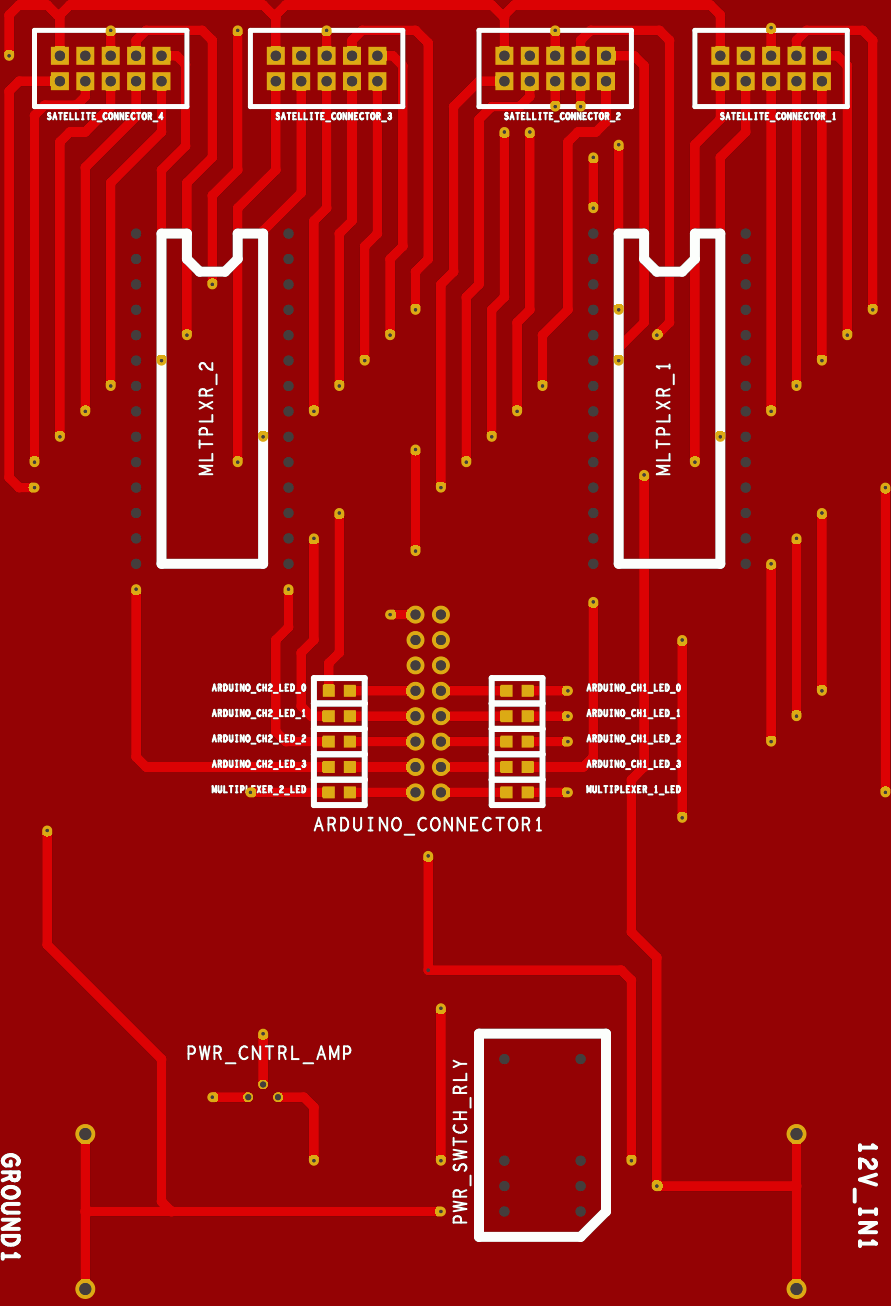
\includegraphics[height=0.2\textwidth,trim={0cm 0cm 0cm 0cm},clip]{pcb-example.png}}{Impedance Analyser Switch}{University of Bath}{I designed and built a 16-channel high-frequency signal switching mechanism. This started with \textbf{\large ECAD} design using \textbf{\large OrCAD}, custom designing 5 PCB's and then manufacturing them including hand soldering surface mount components and finally debugging them an Impedance Analyser (IA). The full system involves a \textbf{\large C\#} application embedded on the IA, using serial communcication to send commands to a custom programmed microcontroller which uses digital pins to control the switching mechanism of the high-frequency relays.}
    \twentyitem{Azure App \vspace{0.1cm} \\ 
\includegraphics[height=0.12\textwidth,trim={6cm 0cm 6cm 0cm},clip]{azure-logo.png}}{Feed: Social Meal Sharing App}{Microsoft Imagine Cup 2018}{For the 2018 Microsoft Imagine Cup I wrote an app for social meal sharing. Using Microsoft \textbf{\large Azure}, a web app was hosted, back-end \textbf{\large C\#} application was created and \textbf{\large MS-SQL} databases were setup which worked together to create a social meal sharing platform. Since the competition I have continued this as a private project hoping to launch this app in the future.}
	\twentyitem{C\# App \vspace{0.1cm} \\ 
\includegraphics[height=0.13\textwidth,trim={0cm 0cm 0cm 0cm},clip]{microsoft-visual-studio.png}}{Large Data Acquisition Application}{Marshall Wace Asset Management}{I wrote a \textbf{\large C\#} application for acquiring large data sets from various sources and streaming them into \textbf{\large MS-SQL} server for use by other departments in the company. It involved multi-threading, task scheduling, custom data structures and cross-platform integration.}
	\twentyitem{MS Kinect \vspace{0.3cm} \\ 
\includegraphics[height=0.03\textwidth,trim={0cm 0cm 0cm 0cm},clip]{kinect-logo.png} \vspace{0.3cm} \\ 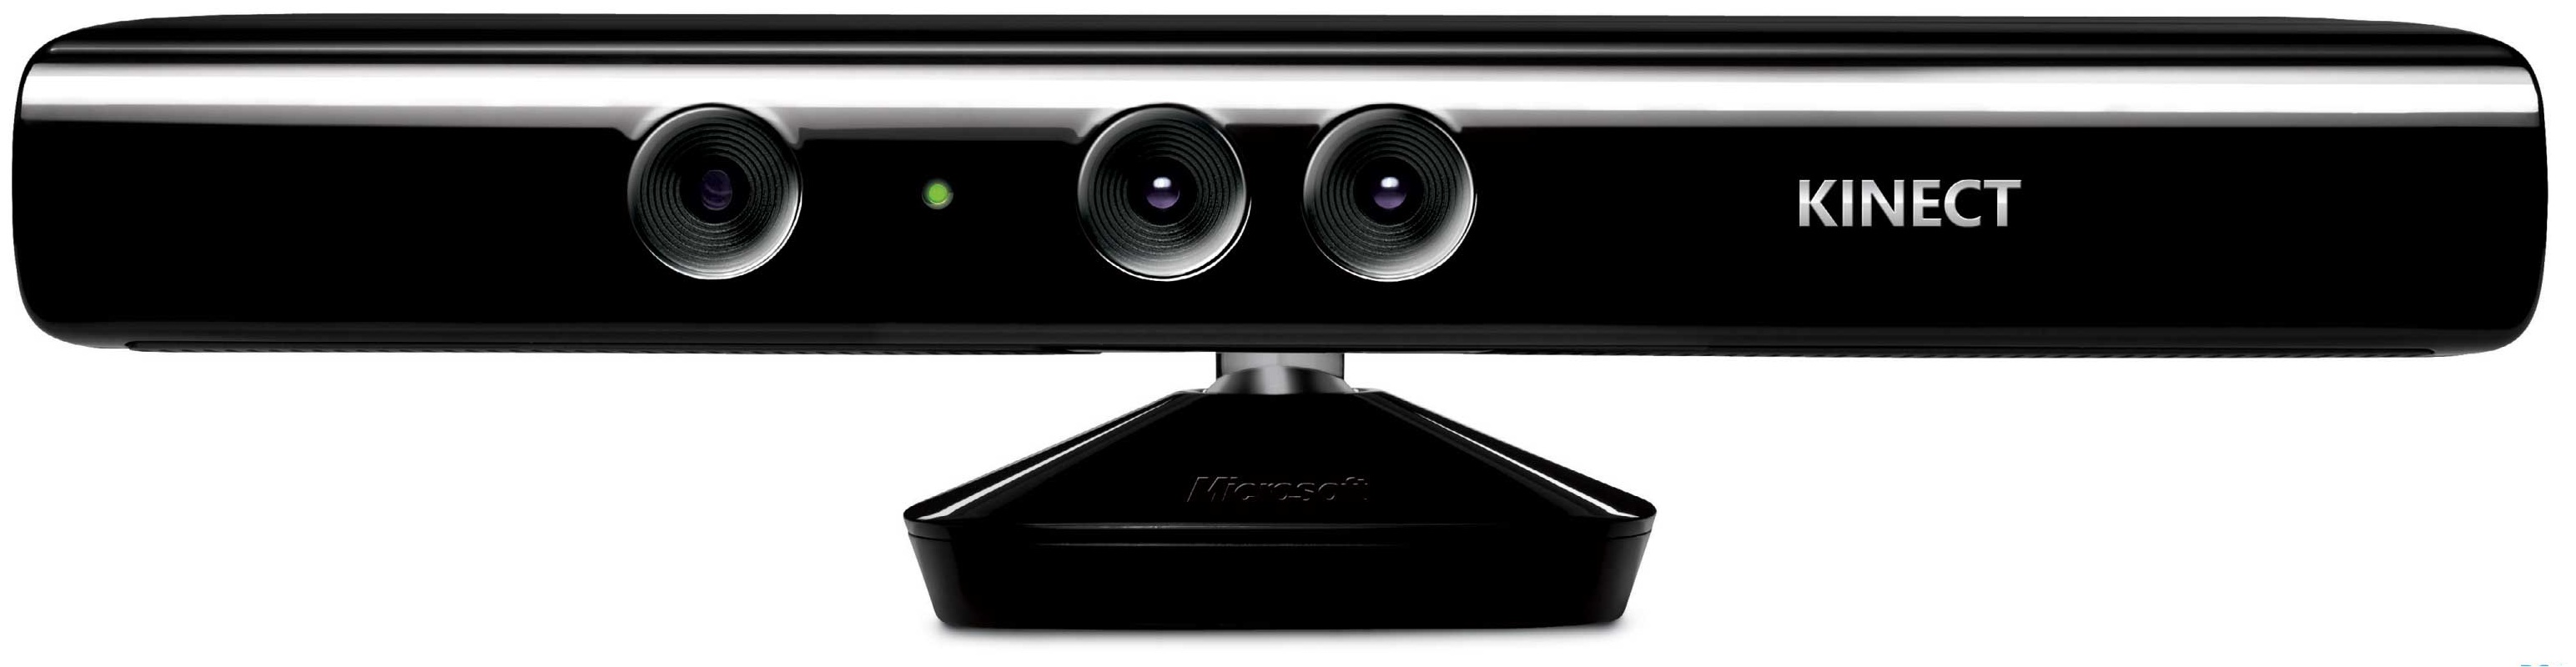
\includegraphics[height=0.035\textwidth,trim={0cm 0cm 0cm 0cm},clip]{kinect-image.jpeg}}{3D Face Detection and Recognition}{University of Bath}{My Masters project was to investigate 3D face recognition using the capabilities of the \textbf{\large Microsoft Kinect}. This involved standard \textbf{\large openCV} face detection algorithms and I developed my own method of recognition for faces using 3D data from the Kinect. The app was written in \textbf{\large C\#}.}
	%\twentyitem{CANbus}{CANbus Test Rig for Hydraulic Actuators}{Parker Hannifin}{I developed a test rig for a  sub-system of hydraulic actuators as part of a larger project we were working on. The hydraulic actuators used the CANbus communication protocol so I built a system that could control them and collect data on how the tests were going. This involved both off-the-shelf components as well as some custom designed circuits which worked together on the test rig.}
	%\twentyitem{<dates>}{<title>}{<location>}{<description>}
\end{twenty}


\section{Hobbies/Skills}
\paragraph{\Large Engineering}
As part of my education I have learnt to use MCAD (Inventor, NX and SolidEdge), lathes, milling machines, laser cutters and many more. I was part of Team Bath Racing as an electrical engineer, building a racing car for the Formula Student competition. I built the wiring loom, mounted electrical components on the car and programmed the ECU.

\paragraph{\Large Sport}
I am a keen skier and in 2015 I qualified as a ski instructor working in New Zealand teaching. I am also a big football fan and I play Sunday League for a local team in Bath as well as in a University league. Finally, I enjoying running and have completed many half-marathons for charities such as MacMillan Cancer Support and Send A Cow.

\paragraph{\Large Film Production}
%From a young age I have had a fascination for film production and video editing. I made many short films as a child and as an adult this hobby has branched into 2 different interests. Firstly, 
I have a huge interest in film production and as part of this I have worked part time as a supporting artist on many feature films and TV series over the last 2 years. It has been great fun and given me new skills not seen in engineering. 
%This has given me an opportunity to see film production from the inside and be part of some great projects.
%Secondly, I still make short films and I have focused on learning visual effects and graphics animation.

\paragraph{\Large University Representation}
During my time at University I have engaged with both the University and Students' Union in a variety of different extra curricular roles. I was a Faculty Representative for 2 years for the faculty of Engineering and Design.
%This involved sitting on committees with staff and students and voicing the student opinion on matters arising within the faculty.
I also spent 2 years on the Executive Committee of the Postgraduate Association as both the Publicity Rep and Engagement Rep.
%This mostly involved organising and running events for postgraduates throughout the year starting with a focused week of activities when they first arrive to a large Ball at the end of each year.
%----------------------------------------------------------------------------------------
\end{document} 
